\begin{enumerate}[label=\thesection.\arabic*.,ref=\thesection.\theenumi]
\numberwithin{equation}{enumi}
\item Plot the polar plot of 
\begin{align}
    G(s) = \frac{1}{(s^2)(s+1)(s+2)}. 
    \label{eq:t1}
\end{align}

\solution
For polar plot we have to plot magnitude of $G(s)$ versus its phase
by varying $\omega$ from 0 to $\infty$.

First substitute, 
\begin{align}
    s = j\omega
\end{align}
Now the magnitude will be
\begin{align}
    |G(j\omega)| = \frac{1}{(\omega^2)(\sqrt{1 + \omega^2})(\sqrt{1+4\omega^2})}
    \label{eq:two}
\end{align}

\begin{figure}[!h]
  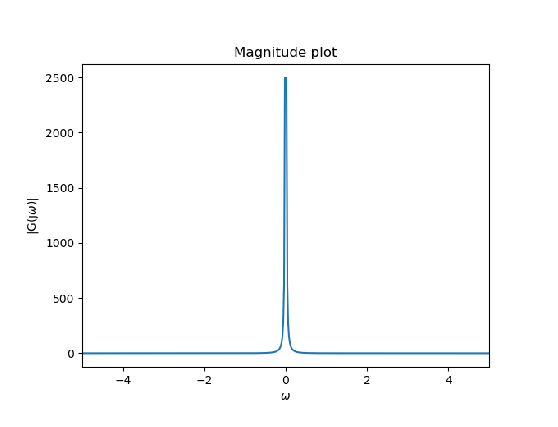
\includegraphics[width=\columnwidth]{./figs/ee18btech11028/magnitude.eps}
  \caption{(a)}
  \label{fig:magnitude}
\end{figure}

Similarly phase $\phi$ can be determined by,

\begin{align}
  \phi = - \tan^{-1}(0) - \tan^{-1}(\omega) - \tan^{-1}(2\omega)
\end{align}
The phase of first term is $\pi$ or can be $-\pi$ since it is a negative real number.
\begin{align}
    \implies \phi = 180\degree - \tan^{-1}(\omega) - \tan^{-1}(2\omega)
    \label{eq:one}
\end{align}

Now we have to sweep $\omega$ from 0 to $\infty$.

So at $\omega = 0$,
\begin{align}
    |G(j \omega)| \xrightarrow{0} \infty 
\end{align}
And phase,

\begin{align}
    \angle {G(j \omega)} = 180 \degree
\end{align}

At $\omega = \infty$
\begin{align}
    |G(j \omega)| \xrightarrow{\infty} 0
\end{align}
 And phase,
\begin{align}
    \angle {G(j \omega)} = 0 \degree
\end{align}

For a complete plot we have to put various values of $\omega$ in 
eq. \ref{eq:one} and eq. \ref{eq:two} for magnitude and phase respectively.
Thus the polar plot looks like, 

\begin{figure}[!h]
  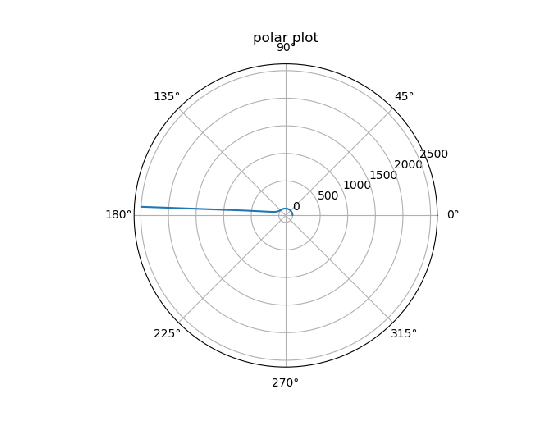
\includegraphics[width=\columnwidth]{./figs/ee18btech11028/polarplot.eps}
  \caption{(b)}
  \label{fig:polarplot}
\end{figure}

To take a closer look at how phase is changing in smaller ranges of $|G(j \omega)|$.
\begin{figure}[!h]
    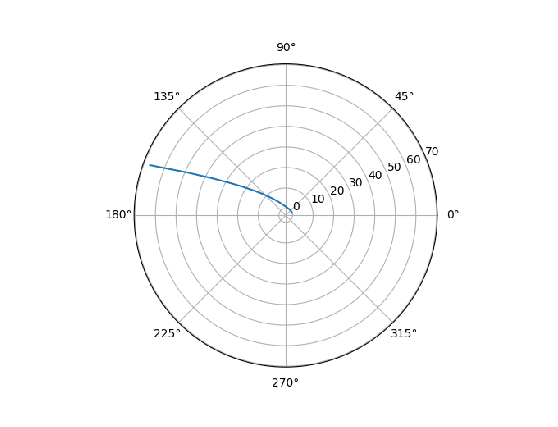
\includegraphics[width=\columnwidth]{./figs/ee18btech11028/polar_plot2.eps}
  \caption{(c)}
  \label{fig:polarplot2}
\end{figure}

The following python code generates  Fig . \ref{fig:magnitude} (a), Fig . \ref{fig:polarplot} (b) and Fig. \ref{fig:polarplot2} (c)
\begin{lstlisting}
codes/ee18btech11028.py
\end{lstlisting}

\textbf{Utility of polar plot in control systems}

Polar plots make it easy to determine the Phase margin (PM) and gain margin (GM) of the system.
This two quantities are substantial for determining the stability of the system.
Please refer to the sections of Gain Margin and Phase margin for definations.

As it is seen in polar plot of \eqref{eq:t1} the graph is not intersecting the 180 $\degree$ line in finite range we will use another transfer function to see the usage of polar plots.

Let's take
\begin{align}
    G(s) = \frac{5}{(s)(s+1)(s+3)}.
    \label{eq:t2} 
\end{align}

The polar plot for this transfer function using the above method looks like,
\begin{figure}[!h]
    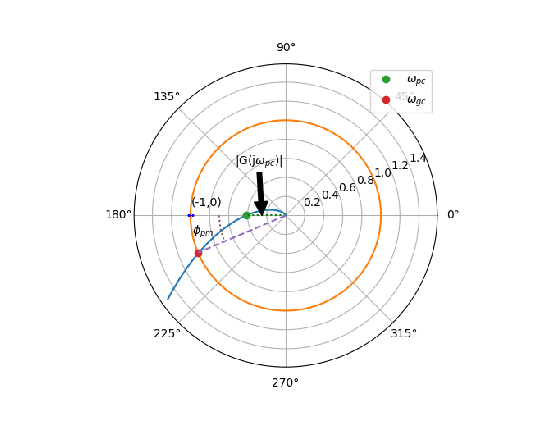
\includegraphics[width=\columnwidth]{./figs/ee18btech11028/example.eps}
  \caption{(d)}
  \label{fig:example1}
\end{figure}

From the plot it's really easy to find GM,
\begin{align}
    GM = \frac{1}{|G(j\omega_{pc})|}
\end{align}
and PM is $\phi_{pm}$ in anti-clockwise direction considered as positive.

Since the polar plot of \eqref{eq:t1} has magnitude of 0 at 180 $\degree$ line it's GM is considered 0.

Now we can deduce the stability of the system by,
\begin{itemize}
    \item If the gain margin GM is greater than one and the phase margin PM is positive, then the control system is \textbf{stable}.
    \item If the gain margin GM is equal to one and the phase margin PM is zero degrees, then the control system is marginally \textbf{stable}.
    \item If the gain margin GM is less than one and (OR) the phase margin PM is negative, then the control system is \textbf{unstable}.
\end{itemize}


We can find phase cross over frequency ($\omega_{gc}$) and gain cross over frequency ($\omega_{gc}$) by putting the magnitudes or phases as mentioned in the legend of \ref{fig:example1} in \eqref{eq:two}
and \eqref{eq:one} respectively.
The following python code generates  Fig . \ref{fig:magnitude} (d),
\begin{lstlisting}
codes/example.py
\end{lstlisting}


\end{enumerate}
